\item \points{4f} \textbf{Implicit regularization of initialization}

We still work with the setup in part (e).
For this sub-question, we use the following datasets:
\begin{center}
	\texttt{src-implicitreg/ir2\_train.csv, ir2\_valid.csv}
\end{center}
Each file contains $d+1$ columns. The first $d$ columns in the $i$-th row represents $x^{(i)}$, and the last column represents $y^{(i)}.$ In this sub-question, we use $d=200$ and $n=40$.

First of all, the gradient of the loss has the following form:
\begin{align}
	\nabla_\theta J(\theta,\phi)&=\frac{1}{n}\sum_{i=1}^{n}((x^{(i)})^\top (\theta^{\odot 2} -\phi^{\odot 2})-y^{(i)})(\theta\odot x^{(i)}),\\
	\nabla_\phi J(\theta,\phi)&=-\frac{1}{n}\sum_{i=1}^{n}((x^{(i)})^\top (\theta^{\odot 2} -\phi^{\odot 2})-y^{(i)})(\phi\odot x^{(i)}).
\end{align}
You don't need to prove these two equations. They can be verified directly using the chain rule.

Using the formula above, run gradient descent with initialization $\theta=\alpha \mathbf{1}, \phi=\alpha\mathbf{1}$ with $\alpha\in \{0.1, 0.03, 0.01\}$ (where $\mathbf{1}=[1,1,\cdots,1]\in\R^{d}$ is the all-1's vector) and learning rate $0.08$. We provide the starter code in \texttt{src-implicitreg/submission.py} and you should implement the \texttt{QP.gradient} and \texttt{QP.train\_GD} functions. Your generated plot should be looking like the following:

\begin{figure}[H]
	\centering
	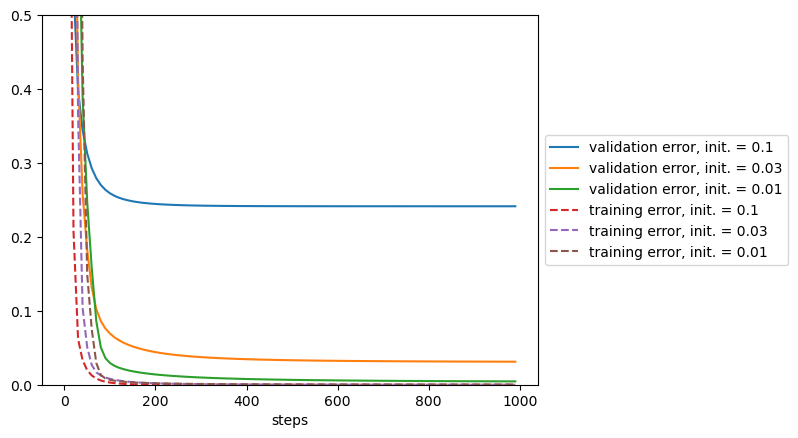
\includegraphics[width=.7\linewidth]{04-implicitreg/implicitreg_quadratic_initialization.png}
\end{figure}

\textit{Remark:} Your plot is expected to demonstrate that the initialization plays an important role in the generalization performance---different initialization can lead to different global minimizers with different generalization performance. In other words, the initialization has an implicit regularization effect. 